\par
In this section, we will discuss the methodology and implementation of solution for lane detection using CNN. We will also elaborate how we used a popular CNN architechure for our use case. Furthermore, we carried out some experiments on our dataset to know whether our choosen CNN architechure is able to detect lanes or not. Before that, we will briefly discuss the technologies and tools used for data gathering, implementation and evaluation of the solution. This chapter is divided into separate sections as mentioned above.

\section{Technology Stack}
\subsection{Unity3D}\label{subsec:unity}
Unity3D is a powerful cross-platform game engine with user-friendly development APIs and environment and is developed by Unity Technologies. It is very easy to begin with and is flexible enough for the expert game developers. Unity is oftenly used to easily create 3D games and applications for mobile, desktop, the web, and consoles. Simulating real-world has saved researchers and scientists has not only provided safe environment but also saved millions of dollars in testing their proposed solutions. Unity3D is also being used in developing interactive simulations and visualizations. Using a real-time 3D virtual world simulated in Unity3d, you can re-enact and test multiple complex scenarios, and understand how you products will perform without putting significant investment in hardware.

\par
Unity3D\cite{unity3d} provides off-the-shelf content to enhance you project and make development easier, organized and faster. These multiple Standard Assets include: Cameras, Characters, Effects, Environment, ParticleSystems, Utility, Prototyping, Vehicles, CrossPlatformInput. Unity’s Asset Store is a library containing free and paid assets created both by Unity Technologies and also members of the Unity community. A lot of variety of assets is available for example models, animations, textures, editor extensions, tutorials or even whole projects.

\subsection{EasyRoads3D}\label{subsec:easyroad3d}
EasyRoads3D\cite{easyroads3d} is a toolset can be imported from Unity's Asset Store and is used to create other infrastructures such as unique road networks and rivers with the riverbed carved in the terrain, using Unity3D. It is a paid asset. You can use fully customizable built-in system of EasyRoads3D or import our own assets to create different road networks from scenic environments to complex urban road networks. It comes with an extremely useful tool of side objects. The side objects tool allows the creation of individual objects like walls, fences, houses, plant vegetation, etc.

\begin{figure}[H]
  \centering
  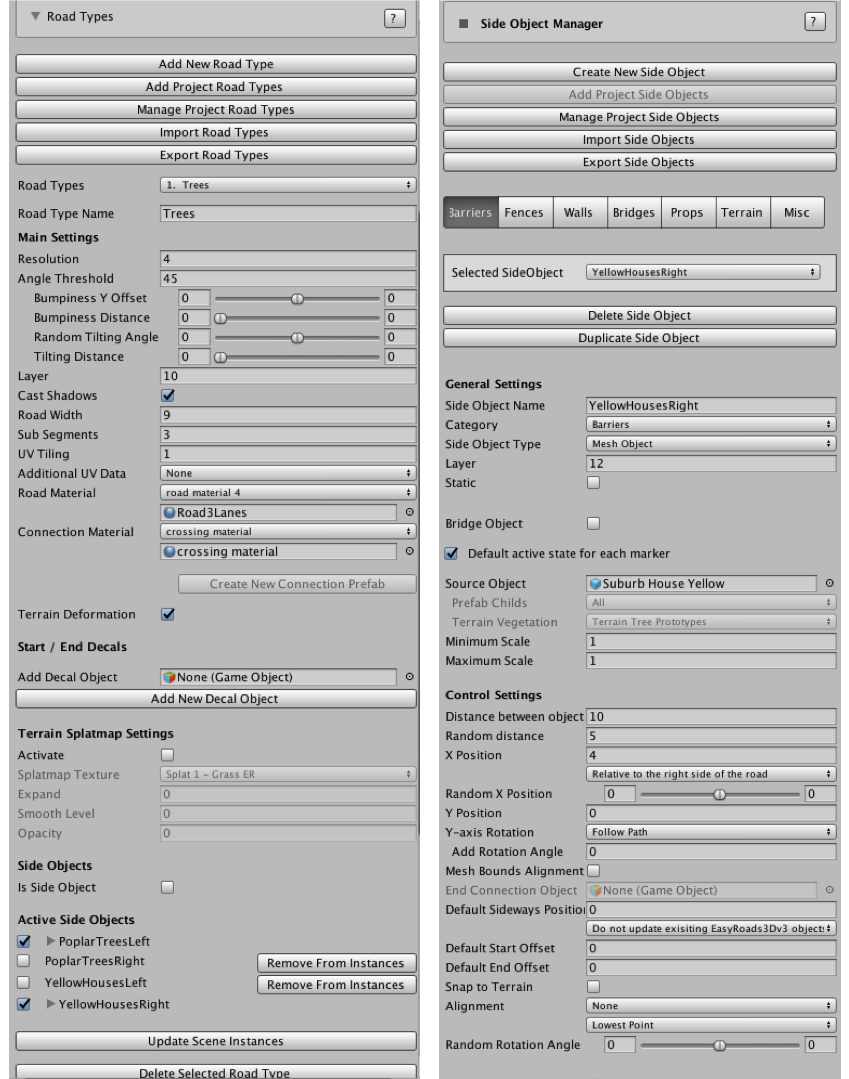
\includegraphics[scale=0.50]{images/Chapter4/easyroad3d.png}
  \caption{EasyRoad3D Unity Inspector}
  \label{fig:remote_ssh}
\end{figure}

\subsection{VSCode}
Visual Studio Code (VSCode)\cite{vscode} is a cross-platform source-code editor developed by Microsoft. It blends the ease of a source code editor with powerful developer tools such as debugging, IntelliSense code completion and integrated terminal. The edit-build-debug cycle is smooth and effortless which means more time to work on your ideas and rather than fiddling with your environment. VSCode is very customizable and extensible by installing extensions to add more features. Some of the notable extensions that I have installed for this project are:
\begin{itemize}
  \item \textbf{Python Extension:} VSCode ships with Javascript, TypeScript, CSS, and HTML language support. Since we are using Python language for training our machine learning model, we can add Python \ref{subsec:python} language support by installing Python plugin\cite{vscode_python}. It not only supports code completion and IntelliSense. IntelliSense is a general term for a number of features, including intelligent code completion (in-context method and variable suggestions) across all your files and for third-party and built-in modules. It shows you methods, class members, and documentation as you type, and allows you to trigger completions at any time. This plugin also allows you to set breakpoints on Python code, inspect data, and use the debug console as you run your program step by step. It also add supports linting of your Python code for potential errors, making it easy to jump to particular section of code and correct different problems.

  \item \textbf{Remote: SSH} 
  The Remote - SSH extension\cite{vscode_remote_ssh} allows you to use and open files and folders hosted on any remote machine with a SSH server as your development environment and take full advantage of VSCode's features. This can help streamline development and troubleshooting in a wide variety of scenarios. For example, you can develop use larger, faster, or more specialized hardware than your local machine or directly develop on deployment machine. Moving between various remote development environments and making changes safely without thinking about the effects of your local machine becomes easy. You can also troubleshoot a program that is deployed anywhere else, such as a customer site or in the cloud.
  \par
  \begin{figure}[H]
    \centering
    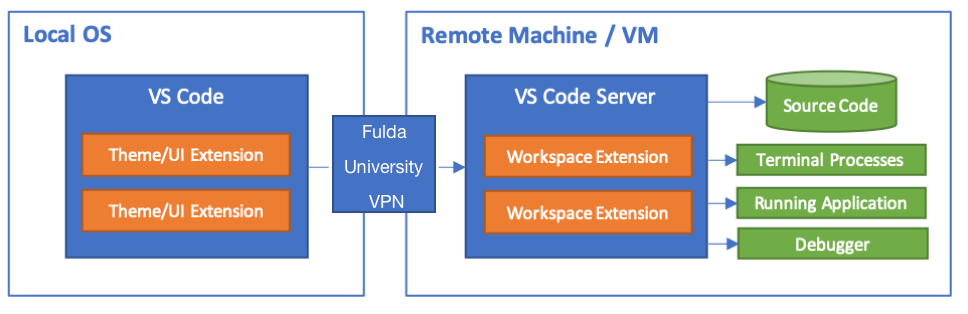
\includegraphics[scale=0.80]{images/Chapter4/architecture-ssh.png}
    \caption{VSCode - Remote SSH plugin Architecture}
    \label{fig:remote_ssh}
  \end{figure}
  In our case, we are using a GPU-heavy cluster machine in Hochschule Fulda for training our machine learning model as my machine has not much resources to train our model with such a large dataset. We could have used Gedit\cite{gedit} or Vim\cite{vim} but it would not have rich features of VSCode. We can only access the cluster through connecting to Hochschule Fulda's VPN. So we set up a simple SSH Tunnel to the cluster through the VPN. We used a \q{configuration file}\cite{config_file} to store the connection as shown in Figure \ref{fig:ssh_connection}, which is supported by OpenSSH, to store all your different SSH connections. Then, we setup \q{key based authentication}\cite{key_based_auth} to login without entering password. Then we can easily use the Remote SSH extension to connect to the cluster. leverage all of the great features of VS Code such as IntelliSense (completions), code navigation, and debugging, as if we were working locally.
  \begin{figure}[H]
      \centering
      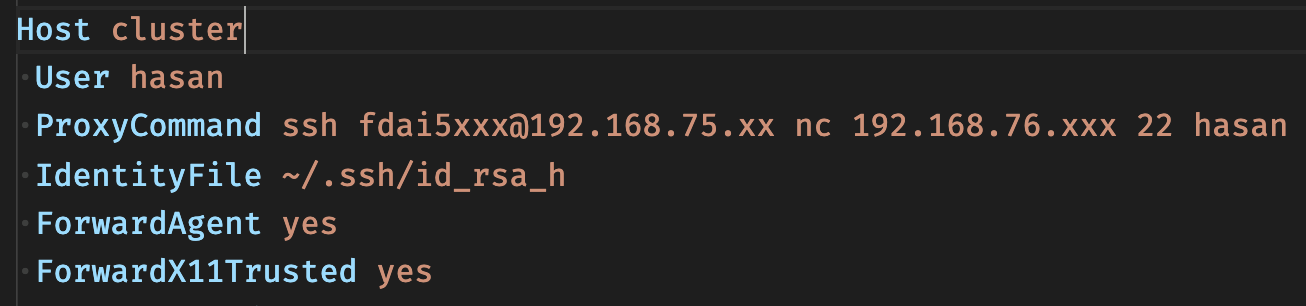
\includegraphics[scale=0.55]{images/Chapter4/ssh_connection.png}
      \caption{SSH connection to GPU-Heavy Cluster}
      \label{fig:ssh_connection}
    \end{figure}
  \end{itemize}

\subsection{Python}\label{subsec:python}
Python is a general purpose, platform independent and high level programming language. It is used for developing desktop GUI applications, web applications and machine learning. Python is the perfect choice for beginners to make your focus on in order to jump into the field of data science and machine learning. It is a stable, flexible, concise, readable and intuitive language with a wide community and full-featured libraries/frameworks which significantly reduces the time required to get your first results. While complex algorithms and versatile workflows stand behind machine learning and AI, the simplicity of Python makes it possible for developers to write robust programs.
% \subsection{Virtualenv}
% vir
\subsection{Tensorflow}
TensorFlow\cite{tensorflow} is basically an open-source Python programming library that contains common machine learning mathematical operations designed to simplify development and deployment of ML powered applications. The library helps users to communicate these mathematical operations as a data flow graph representing the movement of data between operations. The API also speeds up mathematically intensive neural networking and machine learning algorithms on multiple components of CPU and GPU, including optimal CUDA extensions for Nvidia GPU. Tensorflow is the result of Google's long term vision and research in machine learning.
\subsection{Keras}
Keras\cite{keras} is a high-level neural networks API, written in Python. It helps in building, training and testing machine learning models easily using its intuitive high-level APIs with eager execution, which makes for immediate model iteration and easy debugging. The main reasons for using Keras is its user-friendliness, fast learning and model building. You can rapidly prototype a simple or very complex neural networks within a few minutes using Keras. The Model and the Sequential APIs are so powerful that you can do almost everything you may want. Keras provides the benefits of wide adoption and support for a variety of application delivery solutions, compatibility with at minimum five back-end engines (TensorFlow, CNTK, Theano, MXNet, and PlaidML), and strong support for several GPUs and distributed training. Secondly, Keras is backed by Google, Microsoft, Apple, Amazon, Uber, Nvidia, and others. Keras follows the best practices for diminish cognitive load: it exposes a consistent and simple APIs, it reduces the number of user actions required for common use cases, and it provides clear and actionable feedback upon user error.
\subsection{NumPy}
NumPy\cite{numpy} is an open-source general-purpose array-processing Python library. NumPy comprises a multi-dimentional array and matrix data structures. It can be used to run a variety of mathematical operations on arrays such as trigonometric, algebraic and quantitative routines. We have used Numpy a lot to manipulate data. NumPy is an expansion of Numeric and Numarray and Pandas is built around the NumPy array.
\subsection{OpenCV}
OpenCV\cite{opencv} is a cross-platform library which is used to develop real-time computer vision applications and to boost the use of machine perception in the commercial products. OpenCV makes it easy for businesses to use and edit the code. We have used pretty basic features of OpenCV during this project like to load, resize and show images. Some of the things that OpenCV can do out of the box are as following:
\begin{itemize}
  \item Image processing operations.
  \item Video analysis.
  \item Building GUI.
  \item 3D reconstruction.
  \item Feature extraction.
  \item Object detection.
  \item Machine learning.
\end{itemize}

\section{LeNet-5 Architecture}
LeNet-5 is one of the simplest CNN architecture by LeCun et al \cite{lecun1998gradient} in 1998. It has 2 convolutional and 3 fully-connected layers. That is why it has \q{5} in its name. This naming convention is very common for the names of neural networks to be derived from the number of convolutional and fully connected layers that they have. The average-pooling layer as we know it now was called a sub-sampling layer and it had trainable weights. This architecture has about 60,000 parameters. LeNet-5 architecture has become the standard ‘template’: stacking convolutions and pooling layers, and ending the network with one or more fully-connected layers.

\begin{figure}[H]
  \centering
  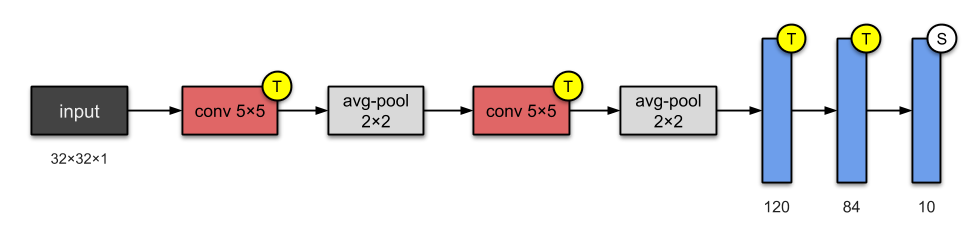
\includegraphics[scale=0.48]{images/Chapter4/lenet5.png}
  \caption{LeNet-5 architecture, based on their paper \cite{lecun1998gradient}}
  \label{lenet5}
\end{figure}
\par
LeNet-5 consists of 7 layers. These layers contain trainable weights. The input, which is by some considered as a part of the architecture, is of a 28x28 pixel image. Each convolutional layer is followed by an average pooling layer. The convolutionary layer recognizes image spatial patterns, such as lines and object parts, and is used to reduce dimensionality through the following average concentration layer. Each convolutional layer uses a 5x5 kernel and processes each output with a sigmoid activation function. The first convolutional layer has 6 output channels, and second convolutional layer increases channel depth further to 16. Nevertheless, the height and width decreased significantly, in combination with this increase in the number of channels. Through increasing the number of output channels, the parameter sizes of the two convolution layers are therefore identical. The two average pooling layers are 2x2 and take non-overlapping stride 2. Expressed in a different way, the pooling layer downsamples the representation to be exactly one-quarter the pre-pooling size. The combination of convolutional and pooling layer generates an output with size given by channel, batch size, height and width. Each example must be flattened in a minibatch before we can move the convolutionary block output to the fully connected unit. Which means, we take this 4 dimensional input and turn it into the 2 dimensional input as expected by fully connected layers. The fully connected layer block of LeNet consists respectively of 3 fully connected layers with 120, 84 and 10 outputs. The 10 dimensional output layer refers to the number of possible output classes because we still carry out classification.
\begin{figure}[H]
  \centering
  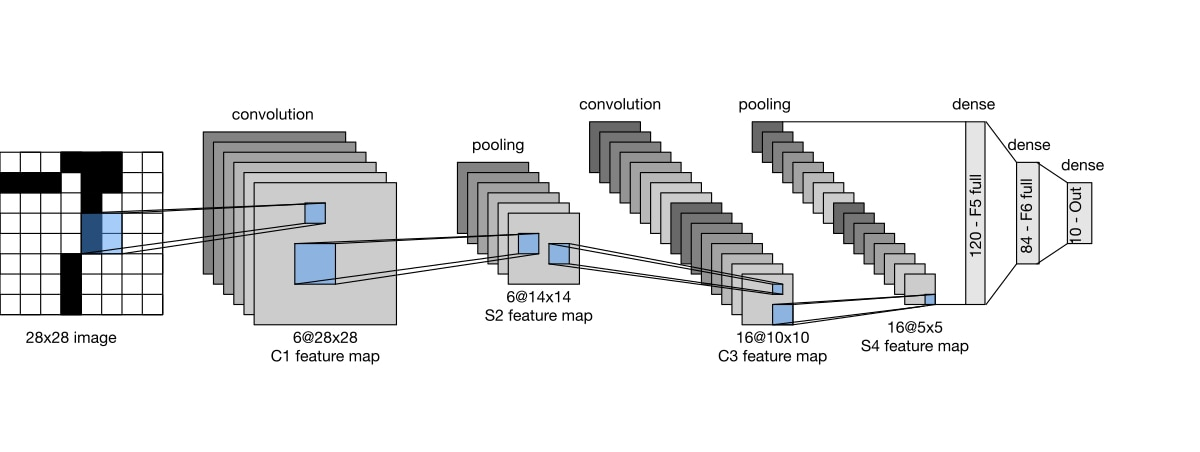
\includegraphics[scale=0.14]{images/Chapter4/lenet.jpg}
  \caption{Data flow in LeNet 5. The input is a handwritten digit, the output a probabilitiy over 10 possible outcomes}
  \label{lenet5}
\end{figure}
\par

\section{Proposed Model}
\par
We have used LeNet-5 architecture because of its simplicity and understandability. Since, our goal is to classify a pixel or region of interest instead of classifying the whole image, we have to tweak the model a little bit. As we have explained above, LeNet-5 model takes an image, we are providing the model a traffic scene image but with pixel coordinates replacing the last pixel in the image. Since our input image size is 256x144, layer's input and output size has been changed. Also we have replaced average pooling layer with max-pooling because max-pooling works better and replaced sigmoid activation function with ReLU activation function because are now known to work more reliably. Because average pooling layer and sigmoid activation function had not been invented at the time when LeChun proposed LeNet-5 \cite{lecun1998gradient}. In the end, the model is trained on the labels that we gathered using segmented image. So our model has 5 output classes namely: lane1 (the rightmost lane), lane2, lane3, lane4 and outside (a pixel that is outside the road).
\begin{figure}[H]
  \centering
  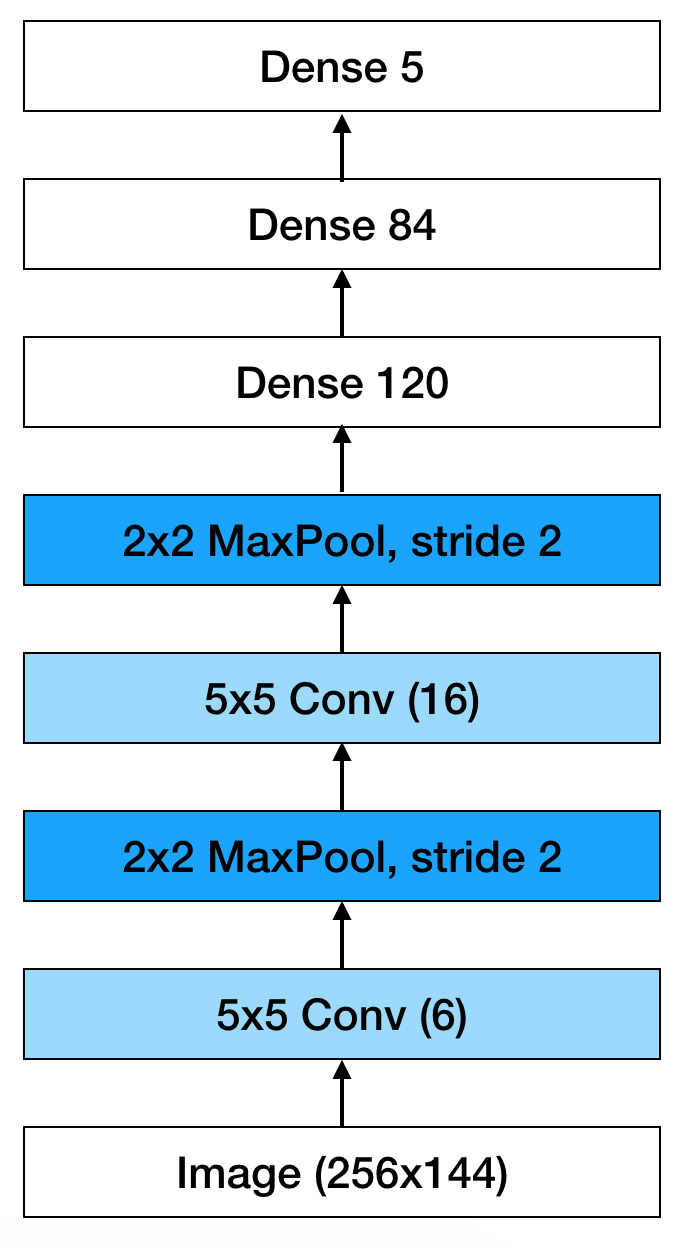
\includegraphics[scale=0.60]{images/Chapter4/proposed_model.png}
  \caption{Compressed notation for our propsed model}
  \label{fig:remote_ssh}
\end{figure}
